\subsection{Filtry AI}

  Filtrowanie obrazów cyfrowych to bardzo popularny i powszechnie stosowany
  obecnie proces. Pozwala wyostrzyć niewyraźne zdjęcie, zmienić kontrast obrazu,
  czy zniwelować szumy tła. W rzeczywistości filtrowanie to nic innego, jak
  operacja matematyczna wykonywana na pikselach. Wykorzystywanie wartości wielu
  pikseli obrazu źródłowego w celu określenia wartości pojedynczego piksela w
  obrazie wynikowym. Sposób w jaki wartości te są pobierane oraz przetwarzane
  określają tak zwane maski. Przyjmują one postać macierzy kwadratowych różnych
  rozmiarów, a przechowywane w nich wartości decydują o wyniku filtracji.

  Poniższy rozdział tej pracy spróbuje udzielić odpowiedzi na pytanie, czy
  sieci neuronowe mogą sprawnie posłużyć w procesie filtrowania obrazów.
  Składa się na niego seria eksperymentów, w których specjalnie dobrane modele
  sieci spróbują odtworzyć wartości masek użytych do przygotowania danych
  treningowych, a następnie wykorzystają je do przetworzenia zupełnie nowych
  obrazów.

  Dane referencyjne składają się z zestawu obrazów przetworzonych za pomocą
  filtrów wbudowanych w bibliotekę \textit{OpenCV} takich, jak filtr Sobela, czy
  sepia.

  Wszystkie modele wytrenowane zostały w oparciu o framework TorchFrame.

  \subsubsection{Filtr Sobela}

    Jednym z podstawowych i najbardziej znanych obecnie filtrów obrazu jest
    filtr Sobela-Feldmana, który zaprezentowany został po raz pierwszy w 1968
    roku na konferencji Laboratorium Sztucznej Inteligencji uniwersytetu Stanforda
    (\textit{SAIL}). Znajduje on przede wszystkim zastosowanie w procesie wykrywania krawędzi
    na obrazach cyfrowych. Sam Irwin Sobel opisuje ten filtr następująco \cite{sobel}:

    \begin{quote}
      Motywacją w rozwijaniu tego rozwiązania było stworzenie wydajnej obliczeniowo
      estymacji gradientu, która byłaby bardziej izotropowa niż popularny wówczas operator
      "Krzyża Roberts'a".
    \end{quote}

    Operator izotropowy to, w kontekście przetwarzania obrazów, operator, którego
    działanie jest równoważne dla wszystkich kierunków na obrazie. Filtr Sobela
    wyznacza przybliżenie gradientu funkcji natężenia obrazu. Dla każdego pojedynczego
    piksela wynikiem jego działania jest wektor gradientu (lub jego długość) wskazującego kierunek wzrostu
    intensywności obrazu, wyznaczony na bazie otaczających wartości ośmiu innych pikseli.

    Na klasyczny filtr Sobela-Feldmana składają się dwie maski:

    \[G_x =
    \begin{bmatrix}
    -1 & 0 & +1 \\
    -2 & 0 & +2 \\
    -1 & 0 & +1
    \end{bmatrix}
    \]

    \[G_y =
    \begin{bmatrix}
    -1 & -2 & -1 \\
    0 & 0 & 0 \\
    +1 & +2 & +1
    \end{bmatrix}
    \]

    $G_x$ odpowiada za filtrowanie krawędzi w pionie, a $G_y$ w poziomie. Obie maski
    mogą być stosowane oddzielnie. Sam proces filtrowania bazuje na konwolucji
    opisanej w ramach sieci splotowych w rozdziale \ref{sieci_splotowe}, polegającej na
    równomiernym przesuwaniu stosowanych filtrów wzdłuż analizowanego obrazu, przy
    jednoczesnym wykonywaniu zdefiniowanych w nich obliczeń w każdym punkcie. Można
    w tym miejscu dostrzec spore podobieństwo pomiędzy klasycznymi maskami i ich zastosowaniem,
    a neuronami wchodzącymi w skład warstw konwolucyjnych sztucznych sieci splotowych. Nie bez powodu
    neurony te nazywane są filtrami.

    W przeprowadzonych doświadczeniach zastosowany został filtr Sobela z
    maską $G_x$. Zbiór uczący wykorzystywany w procesie treningu sieci składał się
    z różnorodnych obrazów dobieranych w sposób losowy. Przykładowe zdjęcia wchodzące
    w skład tego zbioru przedstawia Rysunek \ref{fig:dataset_filters}.

    \begin{figure}[H]
      \centering
      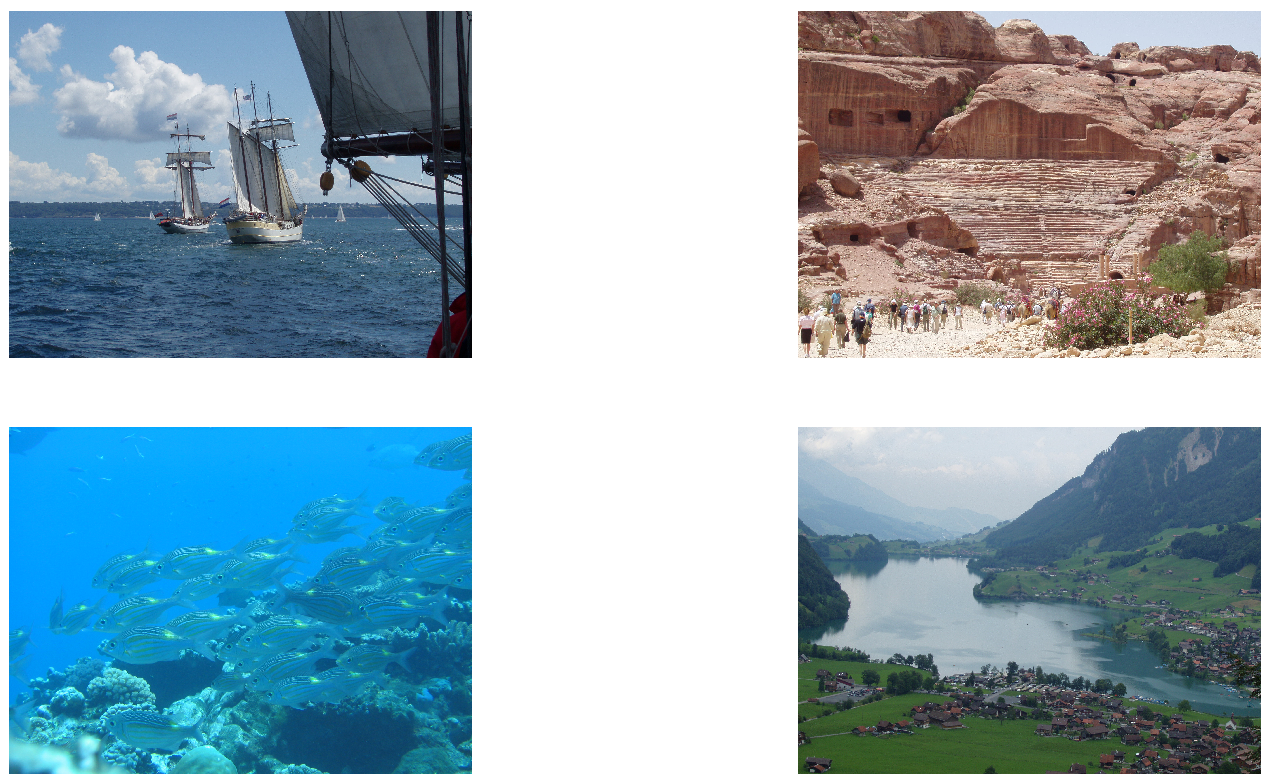
\includegraphics[width=6in]{dataset_filters}
      \caption[Przykładowe obrazy ze zbioru treningowego - źródło: Praca własna]{Przykładowe obrazy ze zbioru treningowego}
      \label{fig:dataset_filters}
    \end{figure}

    Aby mogły właściwie pełnić swoją rolę obrazy treningowe zostały w pierwszej kolejności
    poddane odpowiedniemu przetworzeniu wstępnemu. W ramach tego procesu rozmiar każdego zdjęcia
    zmniejszony został do wymiarów $256x256$ pikseli, a wartości kolorów ograniczone
    do zakresu $<0, 1>$ w celu usprawnienia obliczeń wykonywanych przez sieć m.in.
    poprzez zapobieganie zjawisku eksplodującego gradientu. Dodatkowo w przypadku tego
    filtru zastosowana została konwersja obrazów do formatu czarno-białego, co pozwoliło
    wyodrębnić pojedynczy kanał kolorystyczny z oryginałów. Tak przetworzony zbiór uczący
    podawany był na wejście sieci neuronowej, a rezultaty jej pracy porównywane
    z obrazami na które dodatkowo nałożony został filtr Sobela za pomocą biblioteki
    \textit{OpenCV}. W przypadku obrazów referencyjnych po zastosowaniu filtracji
    konieczne okazało się również przeskalowanie wartości pikseli do przedziału
    $<0, 1>$, ponieważ w sieci zastosowana została funkcja aktywacji \textit{ReLU}, która
    opisana została w rozdziale \ref{funkcje_aktywacji}. Jej charakterystyka
    wyklucza pojawianie się wartości ujemnych, jako rezultatów pracy modelu, co
    w przypadku braku odpowiedniej normalizacji prowadziło do niepoprawnych wyników.

    Sam model sieci składa się w tym przypadku z pojedynczegwo neuronu w warstwie
    konwolucyjnej, filtrującego obraz za pomocą macierzy kwadratowej stopnia
    trzeciego. Odzwierciedla to oryginalną macierz filtracji $G_x$ w stosunku jeden
    do jednego, ponieważ każda z dziewięciu wag sieci odpowiada jednemu polu w tej
    macierzy. Takie podejście pozwala jednoznacznie ocenić stopień odwzorowania
    maski przez sieć poprzez analizę wartości jej parametrów.

    W ramach przeprowadzonych eksperymentów, wypróbowane zostały różne konfiguracje
    hiperparametrów treningowych. Ostatecznie najlepszy rezultat udało się uzyskać
    przy zastosowaniu następującej konfiguracji:

    \begin{itemize}
    \item Funkcja kosztu: \textit{SmoothL1Loss}
    \item Optymalizator: \textit{Adam}
    \item Funkcja aktywacji: \textit{ReLU}
    \item Ilość epok treningowych: 3
    \item Rozmiar pakietu danych: 8
    \end{itemize}

    Efekt działania wytrenowanego modelu przedstawia Rysunek \ref{fig:sobel_result}.

    \begin{figure}[H]
      \centering
      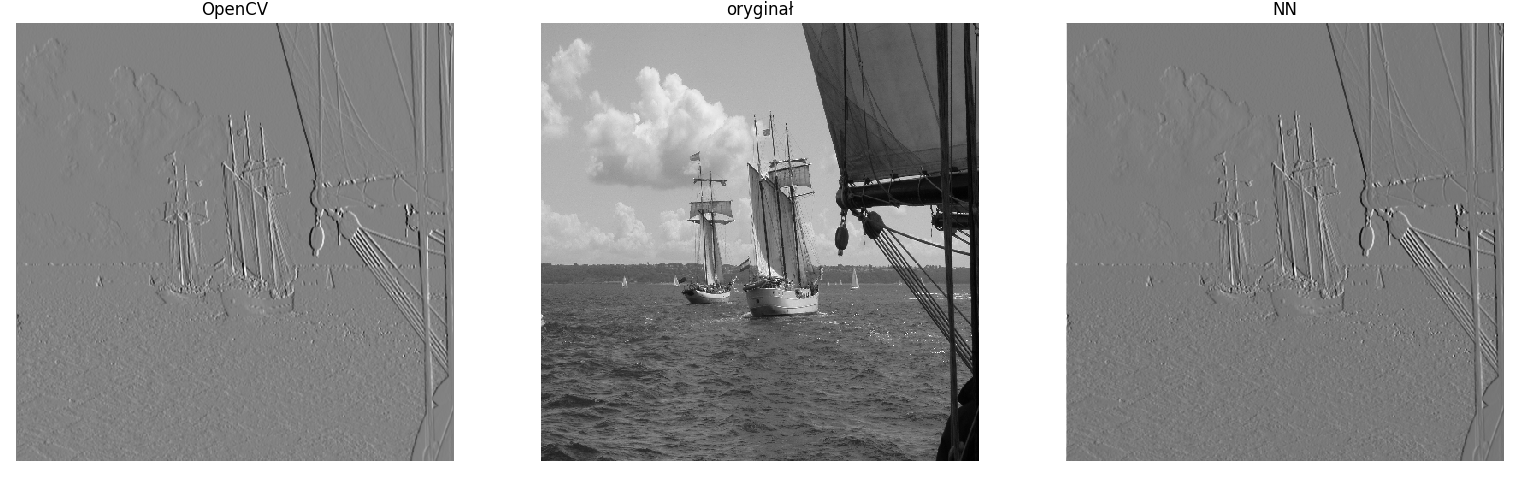
\includegraphics[width=6in]{sobel_result}
      \caption[Działanie filtru Sobela - źródło: Praca własna]{Działanie filtru Sobela}
      \label{fig:sobel_result}
    \end{figure}

    Zgodnie z opisem oryginalne, czarno-białe zdjęcie poddawane filtracji zamieszczone
    zostało na środku. Po lewej stronie przedstawiony został obraz przefiltrowany
    z wykorzystaniem biblioteki \textit{OpenCV}, a po prawej obraz przetworzony przez
    wytrenowany model sieci neuronowej. Wizualnie otrzymane rezultaty są niemal
    identyczne. Zdjęcie wygenerowane przez sieć charakteryzuje się nieco ciemniejszą
    barwą, co może mieć związek z normalizacją danych przeprowadzaną w celu skuteczniejszego
    uczenia sieci. Poprawne rezultaty treningu najlepiej ocenić można analizując
    macierz wag modelu, która przedstawia się następująco:

    \[G_{nn} =
    \begin{bmatrix}
    -0.1135 & -0.0144 & +0.1363 \\
    -0.3239 & -0.0016 & +0.3340 \\
    -0.1199 & -0.0058 & +0.1335
    \end{bmatrix}
    \]

    Porównując uzyskane rezultaty z oryginalną maską $G_x$ łatwo zauważyć można,
    że sieć neuronowa właściwie odtworzyła panujące w niej proporcje. Odpowiednio
    mniejszy rząd wielkości odzwierciedla normalizację danych na których uczony
    był model. Środkowa kolumna składa się w całości z wartości bliskich zeru.
    Kolumna prawa zawiera wartości dodatnie z wyraźną dominacją elementu środkowego.
    Podobnie rozkładają się wartości w kolumnie lewej zawierającej wyłącznie wartości
    ujemne.

    Wskazówką w określaniu poprawności przeprowadzanych treningów może być również
    wykres wartości funkcji kosztu w kolejnych krokach uczenia. Przebieg taki
    przedstawiony został na Rysunku \ref{fig:tensorboard_sobel}.

    \begin{figure}[H]
      \centering
      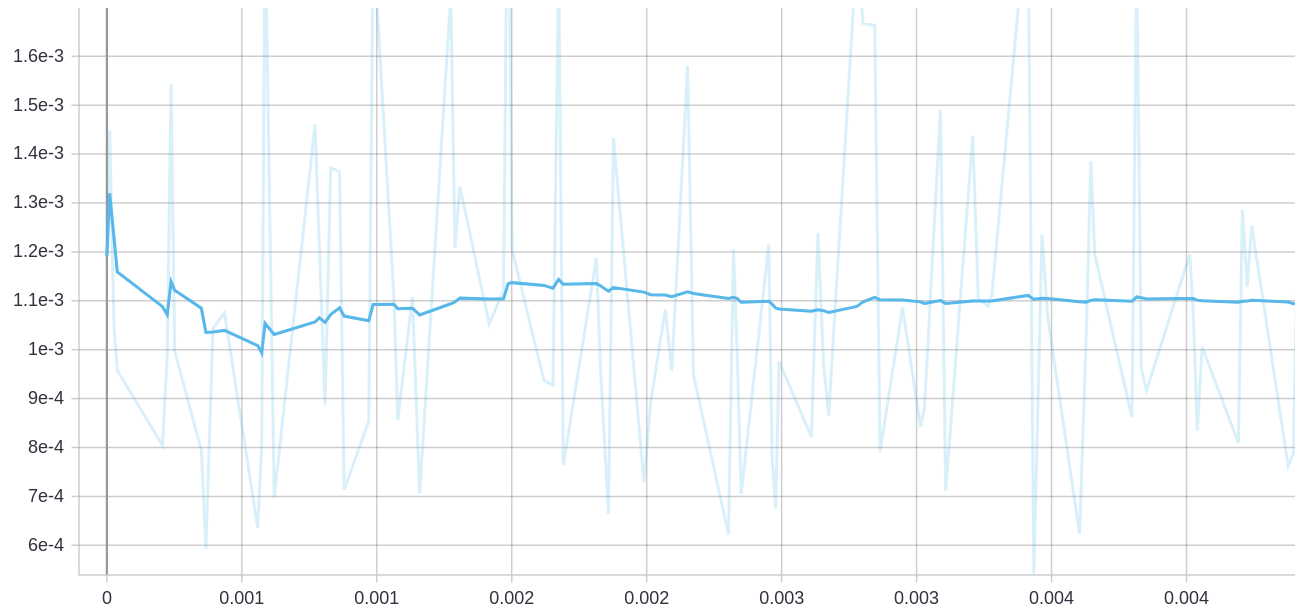
\includegraphics[width=6in]{tensorboard_sobel}
      \caption[Wykres wartości funkcji kosztu w zależności od ilości kroków treningowych - źródło: Praca własna]{Wykres wartości funkcji kosztu w zależności od ilości kroków treningowych}
      \label{fig:tensorboard_sobel}
    \end{figure}

    W początkowej fazie przedstawiona charakterystyka cechuje się znaczącym spadkiem
    wartości, po czym utrzymuje się na stosunkowo stałym poziomie. Jest to spodziewany
    efekt, spowodowany niewielkimi rozmiarami modelu, co przełożyło się na szybkie
    zlokalizowanie globalnego minimum przez zastosowany optymalizator. Warto wspomnieć,
    że zastosowanie tej metryki do analizy działania sieci może być zwodnicze.
    Ciągły spadek wartości funkcji kosztu nie zawsze oznacza wzrost dokładności działania
    trenowanego modelu. Sieć neuronowa może zacząć w zbyt dużym stopniu dostosowywać się
    do dostępnych danych treningowych tracąc zdolność do generalizacji rozwiązania dla
    przykładów spoza tego zbioru. Zjawisko takie nazywane jest przeuczeniem i najczęściej
    objawia się spadkiem dokładności, przy jednoczesnym opadaniu wartości funkcji kosztu.

    Liczne eksperymenty związane z zastosowaniem rozmaitych hiperparametrów wykazały, że
    pomimo niewielkich rozmiarów modelu zlokalizowanie minimum globalnego nie było
    zadaniem trywialnym. Prosty optymalizator, taki jak \textit{SGD} nie był w stanie odnaleźć
    odpowiedniego punktu, a rezultaty jego działania w dużej mierze zależały od
    losowych wartości przypisanych do wag sieci na początku każdej sesji treningowej.
    Dopiero zastosowanie algorytmu adaptacyjnego, jakim jest \textit{Adam} pozwoliło
    uzyskać powtarzalność w osiąganiu właściwych rezultatów. Algorytm \textit{SGD}
    zastosowany został dopiero w końcowej fazie uczenia z bardzo małym krokiem
    treningowym rzędu $\eta = 10^{-8}$, co pozwoliło nieznacznie poprawić uzyskane
    wyniki.

    Olbrzymi wpływ na rezultaty miały również zastosowane sposoby przetworzenia danych
    treningowych, między innymi wspomniane już ograniczenie wartości pikseli
    w przedziale $<0,1>$, tak aby współgrały z zastosowaną funckją aktywacji.

  \subsubsection{Sepia}


  \subsubsection{Filtr górnoprzepustowy}
